Los accesos a la máquina proveen varias formas posibles de ataques: cuánto menos expongan entradas para posibles atacantes, más seguras serán. Por otro lado, se debe tener en cuenta la custodia de las máquinas: quién tiene acceso y cuándo, y si es posterior al último chequeo oficial. Así mismo, se tiene que contemplar y facilitar el acceso a todos los votantes.

\subsection{Acceso a información del hardware}

Para empezar es imprescindible contar con la información completa del sistema a utilizar: software, hardware, flujos, participantes, entre muchas otras cosas. Es necesario para poder auditar previo al hecho electoral, durante y posteriormente al mismo. La importancia de tener la información de cada componente interviniente del sistema, es poder investigar la presencia de vulnerabilidades conocidas o detectar alguna vulnerabilidad en la interacción entre componentes. Un claro ejemplo donde podemos contrastar es el caso de la empresa MSA (Magic Software Argentina), responsable de la votaciones realizadas en Salta y en la Ciudad de Buenos Aires. En su sitio, solo hay información superficial del sistema de votación, en cuanto a las máquinas, nada más que fotos e infografías. Por otra parte, una empresa internacional Smartmatic, dispone en cada producto un documento técnico con información específica de las máquinas\cite{smartmatic}, lo cual genera mayor confianza. Esta última, fue la empresa responsable de las elecciones de La Falda y Marcos Juárez en Córdoba. La empresa afirma que obtuvieron en tiempo récord el escrutinio definitivo, y que fue de 45 minutos apróximadamente\cite{smartmatic:cordoba}.

En el caso de la Ciudad de Buenos Aires, esto se establece en el artículo 24, inciso b, de la Ley 4894. En las etapas previas al acto electoral, es decir, al uso del sistema Vot.ar, se realizaron varias auditorías.
En la auditoría de Claudio Riguetti, por la FCEN, se aclara lo siguiente: “Se destaca la falta de un Manual de Operaciones, que debería incluir todos los aspectos de configuración, instalación, despliegue, mantenimiento, repliegue y obtención y publicación de resultados”\cite{righetti}.

\subsection{Sistemas de control físico y contingencia}

La seguridad física no solo es restringir acceso a los componentes de la máquina, sino que se refiere también a los procedimientos y acciones para que no se violen los sistemas. Si se corrompe una máquina, destruye o algo similar, debería ser fácilmente recuperable o reemplazable. Se deben tener en cuenta mecanismos de contingencia previos y durante la votación. Algunas de las situaciones que se deberían tener en cuenta son incendios en las instalaciones, fallas con la corriente eléctrica, robo del equipamiento, fallas de fábrica o hardware, errores humanos como conteo doble de boletas, atentados, entre otros.

Es importante aprender de errores pasados, por lo que realizar estudios sobre elecciones previas puede aportar mejoras considerables. Para eso es necesario un registro minucioso de cada incidente, registrando casos con la mayor información posible. Un claro ejemplo, es la posibilidad de acceder físicamente a componentes de la máquina, por ejemplo en el caso de la Ciudad de Buenos Aires, la unidad de DVD está accesible, pero sobre todo, un puerto USB que podría permitir cargar algún tipo de script, como BadUSB\cite{votar}.

La EAC\footnote{Election Assistance Commission}, recomienda que ningún ente sea el propio validador de la seguridad de sus máquinas. Se debería de usar el principio de la responsabilidad compartida, es decir, que un agente externo examine y verifique.

Además, que hay que llevar un control estricto del personal, de los componentes que puede acceder y de los permisos sobre los mismos. Indudablemente, un control periódico de las máquinas es necesario, pero también de los lugares donde se lleva a cabo la votación. Al tener toda esa información, ayuda a tener un mejor control ante cualquier eventualidad. Un claro ejemplo, sería que en caso de incendio, como trasladar el equipo, resguardar la información, y cómo reanudar el acto electoral, una vez atacado correctamente el incidente.

Otra recomendación, es en el momento de diseñar el tema del almacenamiento, pensar a largo plazo. Considerar el espacio físico y los medios donde se podría alojar toda la información, políticas de seguridad sobre los mismos. Es necesario para las auditorías posteriores a la votación.

El estudio realizado por VITA acerca de un sistema de votación utilizado en Virginia, USA\cite{vita} registra vulnerabilidades físicas similares a las mencionadas anteriormente acerca de BUE.
La terminal de votación de este sistema, tiene una tapa protectora, que es fácilmente removible. Luego de remover esta carcasa, quedan expuestos puertos usb funcionales. Un ataque realizado por VITA consistió en hacer iniciar un sistema operativo desde una unidad USB y copiar las imágenes de los discos de la terminal.

\subsection{Ejemplo de ``tampering'' de componentes internos}

El componente electrónico de votación en India, llamado EVM, está compuesto por dos partes: la unidad de votación (izquierda \ref{fig:partsIndia}) y la unidad de control (derecha\ref{fig:partsIndia}) que están enlazadas por un cable de 5 metros. Las unidades de votación están realizadas para soportar hasta 16 candidatos. En caso de ser más candidatos, se agrega otra unidad de votación y es posible agregar hasta 4 unidades de votación, dando una capacidad máxima de 64 posibles candidatos. En la unidad de votación, se agrega una hoja indicando que botón representa a cada candidato con el símbolo de su partido político. Para votar, el elector tiene que ser identificado por el presidente de mesa que luego le realiza una marca en el dedo con tinta indeleble para evitar que vuelva a votar y presiona un botón en la unidad de control, permitiendo al elector votar en la unidad de votación. Al realizar esto, se prende una luz en la unidad de votación indicando que el votante está listo para sufragar.

\begin{figure}[H]
  \centering
  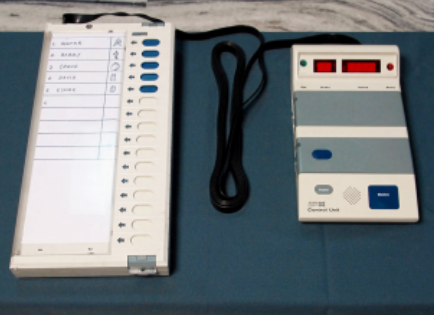
\includegraphics[scale=0.7]{Imagenes/almacenamiento1}
  \caption{Máquina de votación electrónica utilizada en India}
  \label{fig:partsIndia}
\end{figure}

Las vulnerabilidad encontrada en el paper leído es que se puede reemplazar fácilmente algún componente del equipo sea CPU, placas o agregar hardware\cite{india}. Los diseñadores de las EVM podrían haber hecho los ataques más difíciles agregando un mecanismo criptográfico para identificar a los distintos componentes de hardware originales, como un mecanismo de challenge response basado en un secreto contenido en el firmware original.

Uno de los posibles ataques mencionados en el paper es Dishonest Display. Se desarrolló una placa de visualización que puede reemplazar a la placa real en la unidad de control. Normalmente, cuando los votos son contados, la cantidad de votos recibidos por cada candidato figura en el tablero real. Con el ataque, el tablero agrega un microcontrolador que intercepta los votos totales y realiza la sustitución fraudulenta de resultados emitiéndose en el tablero de visualización. Notar que en este ataque hay que realizar un intercambio de un componente de hardware.

\begin{figure}[H]
  \centering
  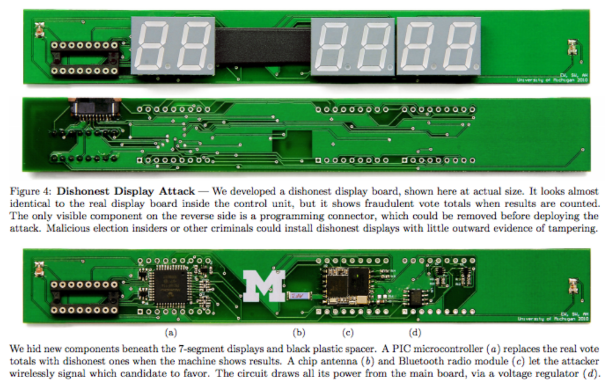
\includegraphics[width=0.8\textwidth]{Imagenes/almacenamiento2}
  \caption{Hardware utilizado}
\end{figure}

Un detalle no menor, es que el recuento de votos de la elección en India se realiza semanas después del sufragio. Por ende, el atacante tiene tiempo para poder realizar el cambio o agregar hardware que le permite realizar el ataque mientras están almacenadas.

Otro ejemplo que afectó a la disponibilidad del sistema de votación fue en las votaciones del Partido Laborista en Israel en el 2008. Las pantallas táctiles de las máquinas fallaban constantemente. El secretario general del Partido Laborista, dijo que las máquinas fueron testeadas por un mes y en cada escenario posible. Otros errores que aparecieron fueron que a algunos votantes les figuraba como que ya habían votado cuando todavía no lo habían hecho. A personas de kibutz, los detectaba como que no estaban habilitados para votar. \cite{haaretz2}
Las consecuencias de estos hechos generaron largas colas para votar, haciendo que gente desista de poder realizar su voto. Finalmente fueron suspendidas hasta el día siguiente donde se volvió al sistema tradicional de voto.
